%Compilation : pdflatex
\documentclass{report}
\makeatletter
\def\@makechapterhead#1{%
  \vspace*{50\p@}%
  {\parindent \z@ \raggedright \normalfont
    \ifnum \c@secnumdepth >\m@ne
      \if@mainmatter
        %\huge\bfseries \@chapapp\space \thechapter
        \Huge\bfseries \thechapter.\space%
        %\par\nobreak
        %\vskip 20\p@
      \fi
    \fi
    \interlinepenalty\@M
    \Huge \bfseries #1\par\nobreak
    \vskip 40\p@
  }}
\makeatother

\usepackage[utf8]{inputenc}
%\usepackage[T1]{fontenc}
\usepackage[a4paper,left=2cm,right=2cm,top=2cm,bottom=2cm]{geometry}
%\usepackage[frenchb]{babel}
%\usepackage{libertine}
\usepackage[pdftex]{graphicx}
\usepackage{color}

%\setlength{\parindent}{0cm}
%\setlength{\parskip}{1ex plus 0.5ex minus 0.2ex}
\newcommand{\hsp}{\hspace{50pt}}
\newcommand{\HRule}{\rule{\linewidth}{0.5mm}}


%\title{Rapport Projet MOGPL}
%\author{Hanane DJEDDAL, Liticia TOUZARI}
%\date{2019-11-24}

%\pagenumbering{gobble} Supprimer numéro de page


\begin{document}
\begin{titlepage}
    \begin{flushleft}
    
\includegraphics[width=11em]{logo.png}\\[1.5cm]
    \end{flushleft}
    %\begin{sffamily}
    \begin{center}
        \textsc{{\LARGE \color{blue} Master Données, Apprentissage et Connaissances-DAC}}\\[5cm]
        \textsc{\Huge{RAPPORT PROJET MOGPL}}\\[1cm]
        \textsc{\Huge{DICE BATTLE}}\\[7cm]
        %\hspace{30pt}
            % Author and supervisor
        \begin{minipage}{1\textwidth}
            \begin{flushleft} \large
            \textsc{\LARGE{Realisé par :}}\\[0.5cm]
            \textsc{Djeddal Hanane}\\
            \textsc{Touzari Liticia}\\
            GROUPE 2\\
            \end{flushleft}
        \end{minipage}
        \vfill
    
        
    \end{center}
   
    
    %\end{sffamily}
  \end{titlepage}
  \tableofcontents
  

  \chapter{Introduction}
  %\addcontentsline{toc}{chapter}{Introduction} \markboth{INTRODUCTION}{} 
  \paragraph{}
  \begin{Large}
  La theorie des jeux est le domaine de mathématique qui permet la modélisation des interactions stratégiques. 
  Dans cet contexte, où plusieurs agents, dites joueurs, cherchent à maximiser leurs gains, le but est de trouver
  une stratégie optimale pour chaque joueur et d'envisager les eventuelles relations liant l'interêt de chauqe 
  joueur, et les possibilités d'un equilibre.\\
  Ce domaine, ayant l'apparence d'un thème restreint, se conforme rapidement à des problèmes d'une grande complexité.\\
  Le but de ce projet est d'etudier les stratégies possibles pour le jeu: Dic-Battle; de comparer expérimentalement ces stratégie
  et à la fin, d'introduire une interface permettant de jouer contre l'ordinateur ou un humain.\\[3.5cm]
  \end{Large}
  \begin{center}
    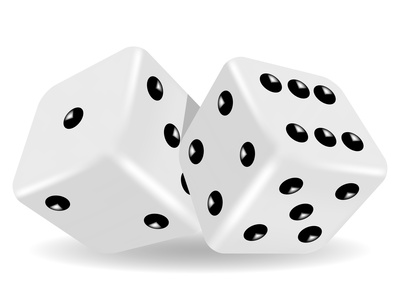
\includegraphics[width=11em]{de.jpg}\\[30cm]
  \end{center}


  \newpage
  \chapter{Description du jeu}
  \paragraph{}
  \begin{large}
  Deux joueurs s'affrontent dans un jeu de dés. Le but est d'être le premier à atteindre au moins
  N points.Le nombre de points marqués est 1 si l'un des dés au moins tombe sur 1,
  dans le cas contraire c'est la somme des dés. On dit qu'un joueur a un gain égal à 1 s'il remporte la partie, un gain égal
  à 0 si la partie est nulle, un gain égal à -1 s'il perd.\\
  Dans ce projet on va étudier deux variante:\\
  - variante séquentielle : les joueurs jouent à tour de rôle;\\
  - variante simultanée : les joueurs jouent simultanément à chaque tour. Dans ce cas si les
  deux joueurs atteignent N points ou plus lors du même tour, c'est le joueur qui dépasse le
  plus les N points qui l'emporte; si les deux joueurs obtiennent le même score, alors ils sont
  ex-aequo.
  \end{large}

  {\let\clearpage\relax \chapter{Probabilite}}
  

  \end{document}